\documentclass[11pt]{article}
\usepackage[utf8]{inputenc}
\usepackage[T1]{fontenc}
\usepackage{amsmath,amssymb}
\usepackage{graphicx}
\usepackage{booktabs}
\usepackage[margin=1in]{geometry}
\usepackage{hyperref}

\title{De la heuristica de independencia al reinforcement learning\\
\large (Notebooks: independence\_gap\_demo + rl\_examples\_demo)}
\author{}
\date{}

\begin{document}
\maketitle

\begin{abstract}
Este documento junta dos ideas:

\begin{enumerate}
  \item \textbf{Heuristica de independencia}. El greedy asume que los
    $Z_i$ son independientes dado el historial $H$ y usa el producto
    de las marginales $\tilde p_i$ para puntuar cada pool. La
    heuristica acierta casi siempre pero a veces falla feo.
  \item \textbf{Reinforcement learning para DAPTS}. Formulamos DAPTS
    como un MDP, resolvemos el valor optimo con \emph{value iteration}
    (identico al DP exacto que ya tenemos), y luego mostramos como
    \emph{Q-learning tabular} se acerca a esa solucion sin conocer el
    modelo de transiciones, solo jugando muchos episodios.
\end{enumerate}

La conexion es que el greedy toma un atajo heuristico porque calcular
$\mathbb{P}(r_t = 0 \mid H)$ exacto es caro; el RL puede aprender una
politica cercana a la optima sin necesitar ese calculo explicito, pero
a cambio de muchos episodios. Son dos puntos de un mismo espectro
"costo vs. precision".
\end{abstract}

%% ====================================================================
\section{Parte 1: La heuristica de independencia}

\subsection{?`Que estamos comparando?}

Cada individuo $i$ esta infectado ($Z_i = 1$) o no ($Z_i = 0$). Despues
de ver el historial $H$ (lista de pools probados y sus resultados),
el greedy mantiene las marginales posteriores
\[
\tilde p_i = \mathbb{P}(Z_i = 1 \mid H).
\]

Para decidir el siguiente pool, el greedy necesita saber cuantos
infectados hay en un pool candidato $t$, es decir la variable aleatoria
\[
r_t = \lvert t \cap Z \rvert = \sum_{i \in t} Z_i.
\]

El greedy aproxima la distribucion de $r_t$ asumiendo que los $Z_i$
son independientes dado $H$. Bajo esa suposicion, $r_t$ tiene una
distribucion Poisson-Binomial con parametros $(\tilde p_i)_{i \in t}$.
En particular:
\begin{itemize}
  \item $\mathbb{P}(r_t = 0 \mid H) \approx \prod_{i \in t} (1 - \tilde p_i)$
    (el caso "clear" que usa el score myopico).
  \item $\mathbb{P}(r_t = \lvert t \rvert \mid H) \approx \prod_{i \in t} \tilde p_i$
    (el caso "todos infectados").
\end{itemize}

\textbf{Problema:} los tests previos introducen dependencias entre los
$Z_i$. Por ejemplo, si antes probamos $t' \subsetneq t$ y $t'$ salio
positivo (al menos un infectado), entonces $t$ tambien tiene al menos
un infectado con probabilidad 1. Pero la heuristica le sigue dando
masa positiva al evento "ningun infectado en $t$".

\subsection{Ejemplo concreto}

Cuatro personas con prior $p_i = 0.5$. Probamos $t' = \{0,1\}$ y el
resultado fue $r' = 1$ (exactamente uno de los dos esta infectado).
Ahora miramos el pool $t = \{0,1,2,3\}$.

Como al menos uno de $\{0,1\}$ esta infectado, $r_t \ge 1$ siempre:
$\mathbb{P}(r_t = 0 \mid H) = 0$. Pero las marginales posteriores de
$0$ y $1$ son $\tilde p_0 = \tilde p_1 = 0.5$ por simetria, asi que
la heuristica da
\[
\prod_{i \in t}(1 - \tilde p_i) = 0.5^4 = 0.0625.
\]

\begin{table}[h]
\centering
\begin{tabular}{lccccc}
\toprule
 & $r_t=0$ & $r_t=1$ & $r_t=2$ & $r_t=3$ & $r_t=4$ \\
\midrule
Exacta      & 0.0000 & 0.2500 & 0.5000 & 0.2500 & 0.0000 \\
Heuristica  & 0.0625 & 0.2500 & 0.3750 & 0.2500 & 0.0625 \\
\bottomrule
\end{tabular}
\caption{Las marginales son correctas ($\tilde p_i = 0.5$ cada una),
pero la forma de la distribucion esta mal porque los $Z_i$ no son
independientes una vez vista la historia.}
\end{table}

\subsection{?`Que tan frecuente es el error?}

Generamos 300 instancias aleatorias con $n = 8$ personas, priors
uniformes en $[0.05, 0.5]$, y $B = 3$ tests seleccionados con el
greedy myopico. Para cada pool candidato de tamano 2 o 3, comparamos
la distribucion exacta (por enumeracion de los $2^n$ mundos) contra
la Poisson-Binomial de las marginales.

\begin{table}[h]
\centering
\begin{tabular}{lrrrrr}
\toprule
$\lvert t \rvert$ & pools & TV media & TV mediana & TV p95 & TV max \\
\midrule
2 & 8400 & 0.024 & 0.000 & 0.217 & 0.500 \\
3 & 16800 & 0.050 & 0.000 & 0.470 & 0.555 \\
\bottomrule
\end{tabular}
\caption{Error (distancia de variacion total) entre la heuristica y
la exacta. La mediana es 0 pero la cola es gorda.}
\end{table}

\textbf{Lectura.} En mas de la mitad de los pools el error es
exactamente cero: la heuristica funciona bien. Esto ocurre cuando el
pool no se traslapa con el historial, o cuando todo el pool ya quedo
determinado por los tests previos. Pero en el top 5\% de los casos
el error llega hasta $\sim 0.47$; el maximo ($\sim 0.55$) aparece
cuando el historial "amarra" a un subconjunto del pool dejando las
marginales individuales intermedias.

\begin{figure}[h]
\centering
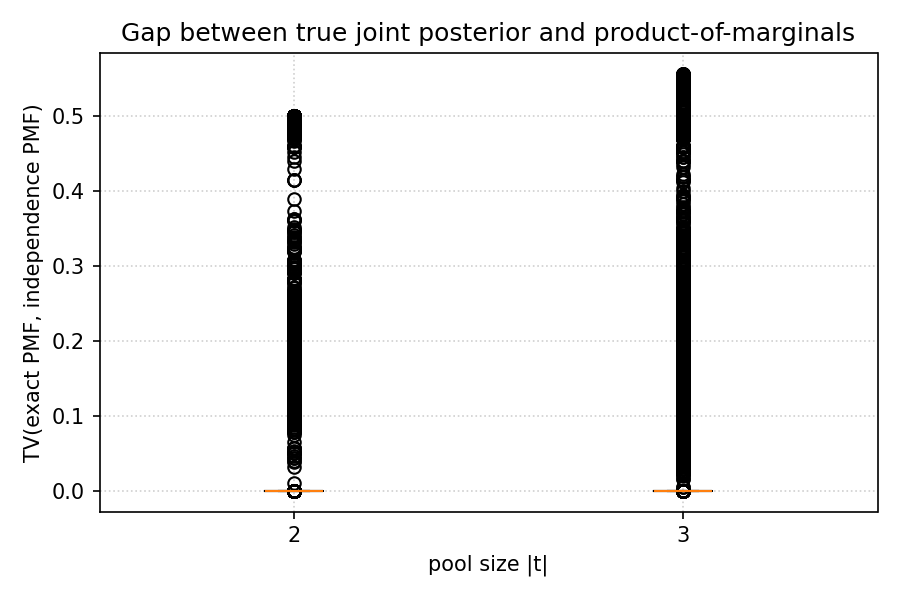
\includegraphics[width=0.75\textwidth]{paper_figs/independence_gap_tv_by_size.png}
\caption{Error entre la PMF exacta y la heuristica, agrupado por
tamano del pool. La caja esta pegada a cero: la mayoria de los pools
tiene error muy pequeno. Los puntos sueltos son casos raros donde el
error llega casi a $0.55$.}
\end{figure}

\subsection{Implicacion}

El score myopico es
\[
\text{score}(t) = \mathbb{P}(r_t = 0 \mid H) \cdot \sum_{i \in t} u_i,
\]
pero se computa con $\prod(1 - \tilde p_i)$. Cuando esa probabilidad
esta sobreestimada (como en los peores casos), el greedy puede
preferir pools que nunca van a "limpiar" nada. Podriamos reemplazar
la heuristica por la probabilidad exacta (via enumeracion por conteo,
o aproximada con Gibbs sobre la query conjunta), pero entonces el
scoring deja de ser barato. Esa tension -- atajo heuristico versus
computo exacto -- es justo el tema de la segunda parte.

%% ====================================================================
\section{Parte 2: DAPTS como MDP y dos ejemplos de RL}

\subsection{?`Que es un MDP?}

Un \emph{Markov Decision Process} es un modelo con:
\begin{itemize}
  \item \textbf{Estado} $s$: lo que sabe el agente en un momento dado.
  \item \textbf{Accion} $a$: lo que puede hacer.
  \item \textbf{Transicion}: dada $(s, a)$, hay una distribucion
    probabilistica sobre el siguiente estado $s'$.
  \item \textbf{Recompensa} $r(s, a, s')$: lo que el agente gana en
    esa transicion.
\end{itemize}

El objetivo es maximizar la suma esperada de recompensas. La
\emph{funcion valor optima} $V^*(s)$ es la recompensa total esperada
si empiezas en $s$ y juegas optimamente. La ecuacion de Bellman dice:
\[
V^*(s) = \max_a \; \mathbb{E}\big[\, r(s,a,s') + V^*(s') \,\big].
\]

\subsection{DAPTS como MDP}

\begin{itemize}
  \item \textbf{Estado}: $s = (k, \text{remaining}, \text{cleared})$.
    Aqui $k$ es cuantos tests ya usamos, $\text{remaining}$ es el
    conjunto de perfiles de infeccion $z$ consistentes con todo el
    historial observado, y $\text{cleared}$ es el bitmask de
    individuos probados sanos.
  \item \textbf{Accion}: un pool $a \subseteq [n]$ con $\lvert a \rvert \le G$
    (el "nada" $a = \emptyset$ tambien es valido).
  \item \textbf{Transicion}: observamos $r = \lvert a \cap Z \rvert$.
    Actualizamos $\text{remaining}$ quedandonos con los $z$
    consistentes con $r$. Si $r = 0$, anadimos $a$ a $\text{cleared}$.
  \item \textbf{Recompensa}: $0$ en pasos intermedios. Al final (paso
    $B$), la recompensa es $\sum_{i \in \text{cleared}} u_i$.
\end{itemize}

Con esta formulacion, $V^*(s_0)$ es exactamente la utilidad esperada
optima del DAPTS; coincide con lo que ya calcula
\texttt{solve\_optimal\_dapts}.

\subsection{Ejemplo 1: value iteration explicita (n=2, B=1)}

Dos personas con $p = (0.3, 0.4)$, utilidades $u = (1, 1)$, un solo
test, tamano de pool $\le 2$.

Acciones: $a \in \{\emptyset, \{0\}, \{1\}, \{0,1\}\}$.

Calculemos $Q^*(s_0, a)$ para cada $a$ con un paso de Bellman:

\begin{itemize}
  \item $a = \emptyset$: nadie se limpia, $Q^* = 0$.
  \item $a = \{0\}$: $r = 0$ con probabilidad $0.7$ (y limpia al $0$
    para utilidad $1$); si no, $r = 1$ y nada se limpia.
    $Q^* = 0.7 \cdot 1 = 0.70$.
  \item $a = \{1\}$: analogo con $p_1 = 0.4$. $Q^* = 0.6 \cdot 1 = 0.60$.
  \item $a = \{0, 1\}$: $r = 0$ con probabilidad $0.7 \cdot 0.6 = 0.42$
    (y limpia a ambos para utilidad $2$); si no, nadie se limpia.
    $Q^* = 0.42 \cdot 2 = 0.84$.
\end{itemize}

La politica optima es probar a los dos juntos:
$V^*(s_0) = \max = 0.84$. \emph{Value iteration} en este caso es solo
un paso de Bellman sobre el estado inicial.

\subsection{Ejemplo 2: value iteration contra el DP exacto (n=3, B=2)}

Tres personas con $p = (0.2, 0.3, 0.4)$, utilidades $u = (1, 2, 1.5)$,
dos tests, $G = 3$.

\begin{itemize}
  \item DP exacto (\texttt{solve\_optimal\_dapts}): $V^* = 2.656000$.
  \item Value iteration explicita sobre el MDP: $V^* = 2.656000$.
  \item Diferencia: $\sim 10^{-16}$ (ruido de punto flotante).
\end{itemize}

Ambos estan haciendo lo mismo: un barrido hacia atras de la ecuacion
de Bellman. La diferencia es solo de vocabulario -- el DP habla de
"subproblemas", el MDP habla de "estados y acciones". Esto ya resuelve
el problema completamente, pero \emph{requiere saber el modelo} (las
probabilidades de transicion). Eso nos lleva al siguiente paso.

\subsection{Ejemplo 3: Q-learning tabular (sin modelo)}

\emph{Q-learning} aprende la funcion valor jugando episodios, sin
necesitar conocer las probabilidades de transicion (por eso se le
dice "sin modelo"). La idea por episodio:
\begin{enumerate}
  \item Sampleamos un perfil verdadero $z$ del prior (nada mas el
    agente no lo ve).
  \item Empezamos en $s_0$ y jugamos $B$ tests. En cada paso, con
    probabilidad $\varepsilon$ probamos un pool al azar (exploracion),
    y con probabilidad $1 - \varepsilon$ escogemos la accion que tiene
    el $Q(s, a)$ mas alto hasta el momento.
  \item Observamos $r$ y pasamos al estado nuevo $s'$.
  \item Ajustamos $Q(s, a)$ hacia el "valor que vimos": la utilidad
    final si $s'$ ya es terminal, o $\max_{a'} Q(s', a')$ si todavia
    queda horizonte.
\end{enumerate}

Para el paso de ajuste usamos un peso $\alpha = 1 / (1 + N(s, a))$
(visitas al par), que es una forma estandar de garantizar que, con
suficientes episodios, el aprendizaje converge.

Sobre la misma instancia (n=3, B=2) corremos 6 seeds con
$\varepsilon = 0.5$ y medimos el valor de la politica aprendida
despues de $500, 1000, \ldots, 50{,}000$ episodios.

\begin{figure}[h]
\centering
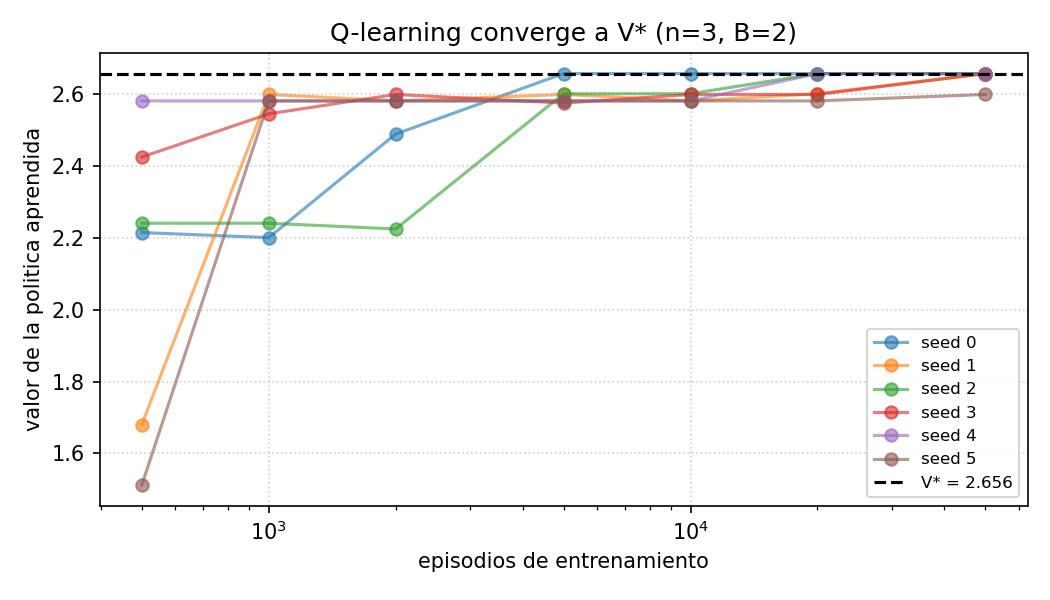
\includegraphics[width=0.85\textwidth]{paper_figs/rl_q_learning_curve.png}
\caption{Q-learning tabular se acerca a $V^* = 2.656$ (linea
punteada). Cada color es un seed. Con $\sim 20{,}000$ episodios casi
todos los seeds ya llegaron al optimo; un seed se queda en $2.598$
(brecha de $\sim 2\%$) incluso a 50k episodios -- en el limite
convergeria, pero aqui sirve como recordatorio de que Q-learning
tabular no "encuentra" la solucion en un numero fijo de episodios:
es un metodo iterativo que acerca, no que resuelve.}
\end{figure}

\subsection{?`Por que importa esto?}

Para $n$ chico, enumerar los $2^n$ perfiles es barato, asi que el DP
exacto gana. Pero a medida que $n$ crece, el numero de estados
explota y no podemos hacer value iteration tabular. Ahi entra el
\emph{function approximation}: Q-learning con redes neuronales (DQN,
PPO, etc.) aproxima $Q(s, a)$ con una red, generalizando entre
estados parecidos. Eso es lo que ya hace
\texttt{classical/rl\_training/PPO\_bucket\_gymnasium\_B*.py} para el
modelo clasico. Adaptar esa infraestructura al modelo aumentado es el
siguiente paso natural (ver \S\ref{sec:siguiente}).

%% ====================================================================
\section{Conexion entre las dos partes}

La heuristica de independencia y el Q-learning tabular estan en
extremos opuestos de un mismo eje:

\begin{center}
\begin{tabular}{lll}
\toprule
Metodo & Conocimiento requerido & Precision \\
\midrule
Heuristica $\prod \tilde p_i$ (greedy) & marginales $\tilde p_i$ & aproximada \\
Counting + greedy & modelo completo & exacta (cara) \\
Gibbs + greedy & modelo completo & aproximada (escalable) \\
Value iteration / DP & modelo completo & optima \\
Q-learning tabular & solo interaccion & en el limite, optima \\
Q-learning + red neuronal & solo interaccion & aproximada (escala) \\
\bottomrule
\end{tabular}
\end{center}

La heuristica es barata pero se equivoca cuando la historia correla a
los miembros del pool. El DP/VI es exacto pero caro. El Q-learning
tabular es un puente conceptual: muestra que, si pudieramos interactuar
muchas veces con el mundo, aprenderiamos la politica optima aun sin
conocer las probabilidades de transicion. Y Q-learning con redes es lo
que permite escalar a $n$ grande aceptando aproximacion controlada.

%% ====================================================================
\section{Siguiente paso}
\label{sec:siguiente}

Direcciones concretas:
\begin{itemize}
  \item \textbf{Greedy con scoring exacto}: reemplazar
    $\prod(1 - \tilde p_i)$ por $\mathbb{P}(r_t = 0 \mid H)$ calculado
    via counting o Gibbs con query conjunta, y medir si reduce la
    brecha contra el optimo.
  \item \textbf{Adaptar PPO a augmented}: reescribir el environment de
    gymnasium con resultado $r = \lvert t \cap Z \rvert$ y actualizacion
    bayesiana por conteo, luego entrenar PPO sobre $n$ grande.
\end{itemize}

%% ====================================================================
\section{Como reproducir}

\begin{verbatim}
python augmented/independence_gap_demo.py
python augmented/rl_examples_demo.py
\end{verbatim}

Los tests unitarios estan en \texttt{augmented/tests.py} (prefijos
\texttt{test\_exact\_pool\_pmf\_*}, \texttt{test\_vi\_*},
\texttt{test\_q\_learning\_*}). La logica esta en
\texttt{augmented/independence\_gap.py} y
\texttt{augmented/rl\_examples.py}.

\end{document}
